\documentclass[letterpaper,12pt]{exam}

\usepackage{ge13}
\usepackage{comment}
\usepackage{booktabs}
\usepackage{hyperref}
\urlstyle{rm}   % change fonts for url's (from Chad Jones)
\hypersetup{
    colorlinks=true,        % kills boxes
    allcolors=blue,
    pdfsubject={NYU Stern course GB 2303, Global Economy},
    pdfauthor={Dave Backus @ NYU},
    pdfstartview={FitH},
    pdfpagemode={UseNone},
%    pdfnewwindow=true,      % links in new window
%    linkcolor=blue,         % color of internal links
%    citecolor=blue,         % color of links to bibliography
%    filecolor=blue,         % color of file links
%    urlcolor=blue           % color of external links
% see:  http://www.tug.org/applications/hyperref/manual.html
}

\newcommand{\NX}{\mbox{\em NX\/}}
\newcommand{\POP}{\mbox{\em POP\/}}

\def\ClassName{The Global Economy}
\def\Category{David Backus}
\def\HeadName{Midterm Examination}

%\printanswers

\begin{document}
\parindent = 0.0in
\parskip = 0.75\bigskipamount
\thispagestyle{empty}%
\Head

\centerline{\large \bf \HeadName}%
%\centerline{March 9, 2005}
\centerline{Revised:  \today}

\bigskip
You have 90 minutes to complete this exam.  Please answer each
question in the space provided and show all of your work.
You may consult one page of notes and a calculator,
but devices capable of wireless transmission are prohibited.

I understand that the honor code applies: I will not lie, cheat,
or steal to gain an academic advantage, or tolerate those who do.

\begin{flushright}
\rule{4in}{0.5pt} \\ (Name and Signature)
\end{flushright}

\begin{figure}[h]
    \centering
    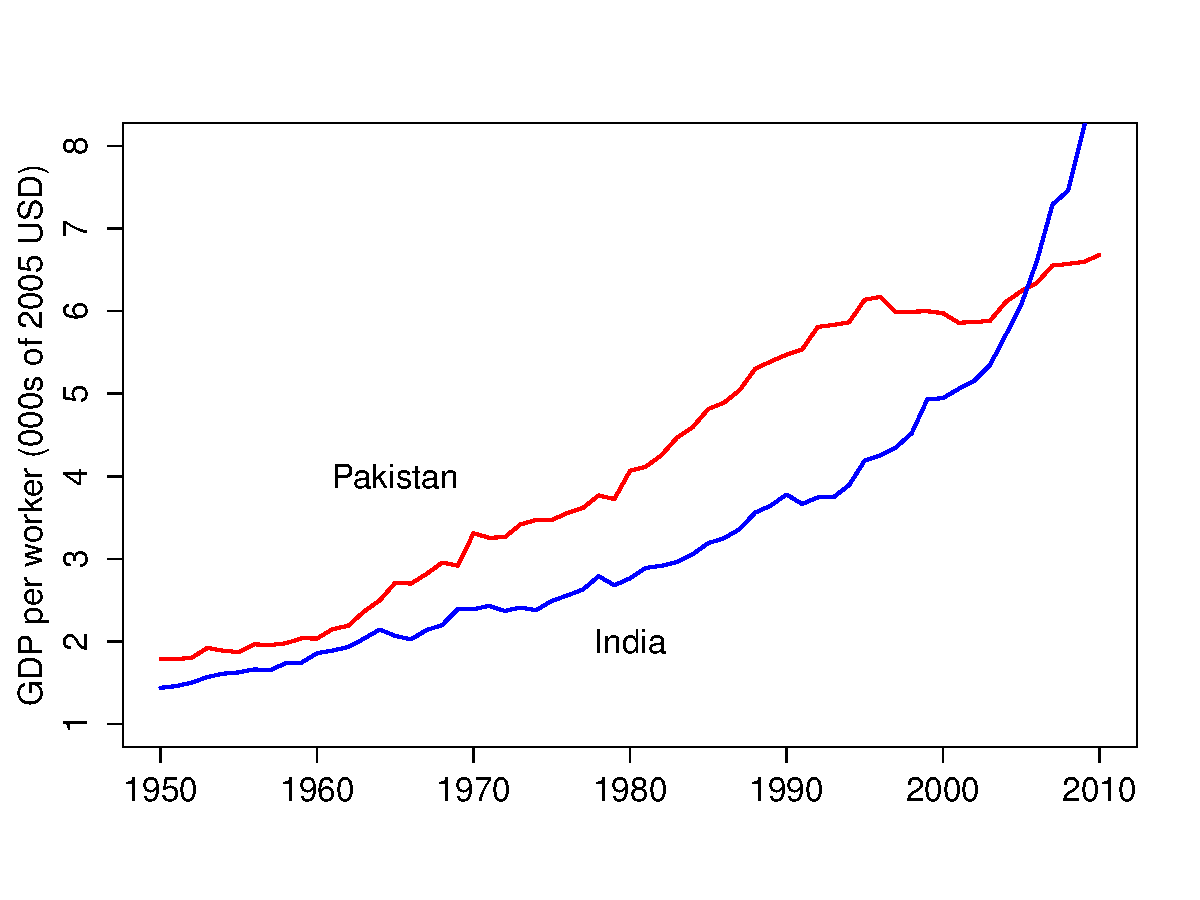
\includegraphics[scale=0.6]{PAKIND_s13_YL.pdf}
    \caption{GDP Per Worker in Pakistan and India.}
    \label{fig:pakistan}
\end{figure}



\begin{questions}
% ======================================================================
\question {\it Prospects for Pakistan.\/}
You have been asked to write a short report on the prospects
for Pakistan:  Can we expect it to grow as India has, or are there
factors that you think will inhibit future economic performance?

Pakistan is a large country, with
an ethnically and linguistically diverse population of 180 million
and an equally diverse geography.
Its level of development after independence in 1947
was comparable to India's.
The Penn World Table estimates that GDP per worker in 1950
was 25\% above India's, with somewhat less difference in
GDP per capita.
Since 1990, however, India has grown rapidly, while Pakistan has not.
See Figure \ref{fig:pakistan} and Table \ref{tab:pakistan}.


The country is now a democracy,
but has alternated democratic and military rule throughout its history.
The Economist Intelligence Unit's Country Report states:
``Pakistan's 1973  constitution established Pakistan as a federal parliamentary
democracy, but it has undergone major amendments to mould the political
system to the wishes of successive political leaders. ...
Still in force before the October 1999 coup launched by General Pervez Musharraf, it
had undergone major amendments, often to legitimise the authoritarian actions
of successive administrations. ...
President Pervez Musharraf
ceded power to a civilian government in early  2008.
In the wake of his resignation the new civilian
government appears likely to amend the constitution once again to limit the
powers of the presidency.
...
The EIU now categorises  Pakistan as a `hybrid regime'
and ranks it 108 (of 167) on its democracy index.''
The EIU adds:
``pervasive official
corruption and increasingly frequent terrorist attacks''
act as a disincentive to foreign investors.
Additional governance indicators from the World Bank
are reported on Table \ref{tab:pakistan-governance}.


\begin{table}
    \centering
    \tabcolsep = 0.3in
    \begin{tabular}{lrrr}
    \toprule
    & India & \multicolumn{2}{c}{Pakistan}  \\
    \cmidrule(r){2-2} \cmidrule{3-4}
    Year     &  $Y/L$ &  $ Y/L $   &  $K/L$   \\
    \midrule
    1990 &  3.780   &   5.473  &   9.040   \\
    2010 &  9.010   &   6.681  &   10.577  \\
    \bottomrule
    \end{tabular}
    \caption{Aggregate data for Pakistan and India.
    The numbers are thousands of 2005 US dollars.
    Source:  Penn World Table, Version 7.1.}
    \label{tab:pakistan}
\end{table}

\begin{table}[t]
    \centering
    \tabcolsep = 0.2in
    \begin{tabular}{lcc}
    \toprule
    & {Pakistan} & India \\
    \midrule
    Voice and accountability	& 26.3 & 59.2  \\
    Political stability	        & 0.5  & 12.7 \\
    Govt effectiveness	        & 22.3 & 54.5 \\
    Regulatory quality	        & 29.9 & 40.3 \\
    Rule of law		            & 20.7 & 52.6 \\
    Control of corruption	    & 15.6 & 35.1 \\
    \bottomrule
    \end{tabular}
    \caption{Governance indicators for Pakistan and India.
    The numbers are percentiles and range from 0 (worst) to 100 (best).
    Source:  World Bank.}
    \label{tab:pakistan-governance}
\end{table}


\begin{parts}

\part Compute continuously-compounded annual growth rates of GDP per worker
for Pakistan and India for the period 1990-2010.
Which is higher?
(10~points)

\part Identify the sources of growth in Pakistan over the same period.
(This is an indication that you should do the usual growth accounting calculations.)
Why has growth been so slow?
(15~points)

\part Use the information provided to assess Pakistan's prospects.
Do you see it growing like India or more slowly?  Why?
(10~points)
\end{parts}

\begin{solution}
\begin{center}
    \tabcolsep = 0.2in
    \begin{tabular}{lrrrr}
    \toprule
    & India & \multicolumn{3}{c}{Pakistan}  \\
    \cmidrule(r){2-2} \cmidrule{3-5}
    Year     &  $Y/L$ &  $ Y/L $   &  $K/L$  & $A$  \\
    \midrule
    1990 &  3.780   &   5.473  &   9.040   & 2.627 \\
    2010 &  9.010   &   6.681  &   10.577  & 3.044 \\
    Growth rate (\%) & 3.343  & 0.997 & 0.785 & 0.735 \\
    \bottomrule
    \end{tabular}
\end{center}

\begin{parts}
\part Complete table of calculations above.
The annual growth rate of Pakistan's GDP per worker is
\begin{eqnarray*}
    \gamma_{Y/L} &=& [\ln (6.681) - \ln(5.473)]/(2010-1990) \;\;=\;\; 0.997 \%.
\end{eqnarray*}
The others are computed the same way.
We see growth rates of (roughly) 4.3\% in India and 1.0\% in Pakistan,
which is a huge difference over 20 years.
You can see the result in Figure \ref{fig:pakistan}.

Grading:  5 points for each calculation done correctly.

\part Growth accounting involves this equation:
\begin{eqnarray*}
    \gamma_{Y/L} &=& (1/3) \gamma_{K/L} + \gamma_{A} .
\end{eqnarray*}
With the numbers above, we have
\begin{eqnarray*}
    0.997 &=& (1/3) 0.785  + 0.735 .
\end{eqnarray*}
We see that most of the growth has been due to productivity $A$,
but the total is small.
Evidently there's little productivity growth or capital formation in Pakistan,
with the result that there's little growth in output per worker.

Grading:  3 points for noting the growth accounting equation,
3 for each of the numbers in it,
3 more for interpreting the results sensibly.

\part How does Pakistan look to you?
The political history and governance indicators all show
that Pakistan's institutions work less well than India's.
It's not hard to imagine that political instability,
lawlessness, and corruption discourage investment
and productivity improvements.

Grading:  10 points for linking slow growth to the
political history and governance indicators.
\end{parts}
\end{solution}


%\pagebreak \phantom{xx} \pagebreak %\phantom{xx} \pagebreak
% ======================================================================
\question {\it Foxconn's next frontier.\/}
Hon Hai Precision Industry Co. Ltd. (``Foxconn'') is a Taiwan-based manufacturer that makes
products for Apple, Intel, Sony, and others.
Known for its plants in China, including one in Shenzhen that makes iPads,
it also has operations in Brazil, Malaysia, Mexico, and other locations.

With wages rising rapidly in China, Foxconn is exploring other locations.
As a private consultant, you have been asked to write a short report
outlining the advantages and disadvantages of locating in Thailand and Vietnam
and to compare both to China.
You collect the information in Table \ref{tab:ctv} and begin your report.

\begin{table}[h]
\centering
\tabcolsep = 0.1in
\begin{tabular}{lrrr}
\toprule
Indicator & China & Thailand & Vietnam \\
\midrule
\multicolumn{2}{l}{\it General} \\
GDP per capita  (2005 USD) &  8400 & 9200 & 3500  \\
Doing Business overall (percentile) & 50.8  &90.3 & 46.5 \\
World Economic Forum overall (percentile) & 80.0 & 73.6 & 47.9\\
\midrule
\multicolumn{2}{l}{\it Governance} \\
Political stability (percentile)  &  25.0 & 16.5 & 52.8 \\
Govt effectiveness (percentile)   &  60.7 & 59.7 & 45.0 \\
Regulatory quality                & 45.5  & 56.4 & 29.4\\
Rule of law                       & 41.8 & 48.8 & 39.9 \\
Control of corruption (percentile) & 30.3 & 43.6 & 33.6  \\
\midrule
\multicolumn{2}{l}{\it Labor} \\
Minimum wage (USD per month) &  204 & 118 & 65 \\
Severance after 10 years (weeks of pay) & 43 & 50 & 43 \\
Labor market efficiency (percentile) & 71.5 & 47.2 & 64.6 \\
Literacy (percent of adults)        & 94 & 94 & 93 \\
Years of school (adults)        & 8.2 & 7.5 & 6.4 \\
\midrule
\multicolumn{2}{l}{\it Infrastructure and trade} \\
Infrastructure quality (percentile)  & 66.7 & 68.1 & 34.0 \\
%\midrule
%\multicolumn{2}{l}{\it International trade} \\
Export documents required (number) & 8 & 5 & 6\\
Export delay (days) &  21 & 14 & 21  \\
Export cost (USD per container) &  580 & 585 & 610 \\
\bottomrule
\end{tabular}
\caption{Institutional indicators for China, Thailand, and Vietnam.
Percentiles range from 0 (worst) to 100 (best).
Sources:  Penn World Table, World Economic Forum, World Bank, Doing Business.}
\label{tab:ctv}
\end{table}


\begin{parts}
\part Which of these indicators are most important to your venture?
How do the two countries compare on them?
(10~points)
\part Which country or countries would you recommend to your clients?
What are the primary challenges they would face?
(10~points)
\end{parts}

\begin{solution}
This is a more qualitative question, but here's an outline
of what a good answer might look like.
A good answer should put some structure on the analysis,
not simply list what's in the table.

\begin{parts}
\part If you build a plant in another country, you'll be concerned
with overall institutional quality,
property rights (whether the government might steal the plant),
labor cost and quality,
labor market institutions,
and the challenges of exporting your product.
There's no clean link to the indicators, but you might guess that
property rights would be related to the governance indicators,
esp political stability and the rule of law.
The labor indicators obviously address concerns with labor.
And infrastructure and trade address the challenges of exporting.

As a rough guide:
\begin{itemize}
\item Overall:  It's interesting that Doing Business rates
Thailand highest, but the World Economic Forum rates China highest.
And the differences are large.  In the real world,
this would call for a closer look.
Ditto the source of political instability in Thailand.
\item Property rights and overall:  Thailand looks a bit better than the
others on Control of Corruption and Rule of Law, Vietnam looks better
on Political Stability.
\item Labor cost and quality:  Vietnam is considerably cheaper than the other two,
if we use GDP per capita or the minimum wage as rough guides to wages.
Literacy is similar in the three countries, China is highest, and Vietnam lowest,
on education.
\item Labor institutions:  The World Economic Forum ranks China highest,
and Thailand lowest, on overall labor market efficiency.
Another thing that's worth a closer look.
Severance looks similar.

\item Exporting:  cost and delay look similar, but Vietnam
has the worst infrastructure.
You'll want to look into this, see what aspects of the infrastructure
are likely to affect you.
\end{itemize}

Grading:  10 points for a clear list of issues and
a logical argument that connects
the institutions to the demands of the business.
Partial credit for part thereof.

\part

To me, they both look like reasonable candidates.
For Thailand, I'd want to look closer at political stability,
see what that represents and think about how it would affect me.
For Vietnam, I'd want to look closer at infrastructure.

Grading:  10 points for a logical argument
that flows from your earlier analysis and identifies
the key issues in Thailand and Vietnam.
\end{parts}
\end{solution}

%\pagebreak \phantom{xx} \pagebreak \phantom{xx} \pagebreak
% ======================================================================
\question {\it Short questions.\/}
%
\begin{parts}
\part XYZZY Partners offers business consulting
services worldwide from its US headquarters.
In 2012, sales were 235 (million dollars),
of which 60 came from clients in other countries.
Expenses included labor compensation of 150, rent of 35,
and materials of 25.
Any surplus goes to the firm's partners.
They also purchased enterprise resource management software
from German software giant SAP for 85,
which they will treat as a capital expenditure
and amortize over ten years.

What was the firm's contribution to US GDP?
(10~points)


\part In Ricardo's model, what is the impact of trade on jobs?
(10~points)

\part When an unemployed person stops looking for work,
what happens to the unemployment rate?
The employment rate?
The labor force?
(10~points)

\part Consider the statement:  ``In financial markets it's important
to protect lenders.  Otherwise, both borrowers and lenders lose.''
Do you agree or disagree?  Why?
(10~points)

\part Consider the statement:
``It's not necessary for a country to save in a global economy.
Firms can finance all the investment they want in
global capital markets.''
Do you agree or disagree?  Why?
(10~points)


\end{parts}

\begin{solution}
\begin{parts}
\part Value added by XYZZY is sales of 235 minus materials of 25,
for a total of 210.  None of the other numbers are relevant.

\part In Ricardo's model, the amount of work (jobs, hours) is
the same with and without trade.
As we said in class:  trade is about which jobs, not the number of jobs.

\part We divide the adult population into these categories:
A = working, B = unemployed (not working, but looking for work),
and C = neither working nor looking for work.
In the example, the person has left B and entered C,
so B falls by one and C rises by one.
The unemployment rate B/(A+B) it falls.
The employment rate is A/(A+B+C), so it stays the same.
The labor force A+B falls.

\part The idea is that if we don't protect lenders, they will simply
decide not to lend.
That hurts borrowers who have profitable projects that go unfunded.
In class we illustrated this with a simple game, but it's not necessary to
go through that.

\part This is a call to apply the flow identity,
\begin{eqnarray*}
    S &=& I + \NX .
\end{eqnarray*}
If investment $I$ is greater than saving $S$,
then firms can finance the difference by raising money in
international capital markets ($\NX < 0$).
As an example:  when Norway developed oil fields in the North Sea,
it didn't need to finance that all at home,
it could access international markets.
And it did.
Ditto Ghana today.

\end{parts}
%
Grading:  10 points for clear statements along the same lines as these answers.
\end{solution}

\end{questions}

%\pagebreak \phantom{xx} %\pagebreak \phantom{xx}

\vfill \centerline{\it \copyright \ \number\year \ NYU Stern
School of Business}

\end{document}
